\xiti
\begin{xiaotis}

\xiaoti{用厚纸做一个正三棱锥或正四棱锥的模型。}

\xiaoti{已知底面边长是 $a$,高是 $h$。 求下列棱锥的侧棱长和斜高:
    (1)正三棱锥;(2)正四棱锥;(3)正六棱锥。
}

\xiaoti{已知正六棱锥的底面边长是 4 cm,侧棱长是 8 cm。求它的侧面和底面所成的二面角。}

% TODO: wrapfigure 在这里无法正常使用
\begin{minipage}{11cm}
    \jiange

    \xiaoti{已知正三棱锥的底面边长为 $a$。求过各侧棱中点的截面面积。}

    \xiaoti{求证:平行于三棱锥的两条相对棱的平面截三棱锥所得的截面是平行四边形。}

    \xiaoti{棱锥的底面积是 $150\;\pflm$,平行于底面的一个截面面积是 $54\;\pflm$,
        底面和这个截面的距离是 12 cm,求棱锥的高。
    }

    \xiaoti{画一个底面边长是 4 cm,高是 8 cm 的正六棱锥的直观图(选择适当比例尺)。}

    \xiaoti{正三棱锥的底面边长是 $a$,高是 $2a$,计算它的全面积。}

    \jiange
\end{minipage}
\quad
\begin{minipage}{4cm}
    \centering
    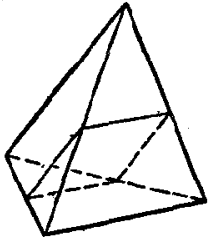
\includegraphics[width=3cm]{../pic/ltjh-ch2-xiti8-05.png}\\
    (第 5 题)
\end{minipage}

\xiaoti{一座仓库的屋顶呈正四棱锥形,底面的边长 2.7 m,侧棱长 2.3 m,
    如果要在屋顶上铺一层油毡纸,需要油毡纸多少平方米?
}

\xiaoti{要做一个正六棱锥形的铁烟囱帽,底口边长 40 cm,高是 50 cm,需要多少平方米铁皮?}

\xiaoti{一个棱锥所有的侧面与底面所成的二面角都等于 $\alpha$,那么
    $$ S_\text{侧} = \dfrac{S_\text{底}}{\cos\alpha} \juhao $$
}

\end{xiaotis}

